\documentclass{snedecorbeamer}

%% Slide numbers
\usepackage{appendixnumberbeamer}

%% References
\usepackage{cleveref}

%% Figures
\usepackage{subcaption}

%% Captions
%%% Small font
\captionsetup{font=tiny}
%%% Remove caption
\setbeamertemplate{caption}{\raggedright\insertcaption\par}

%% Footnotes
%%% Small font https://tex.stackexchange.com/a/146021
\setbeamerfont{footnote}{size=\tiny}

%% Symbol resizing
\usepackage{scalerel}

%% Diagrams
%%% General tikz preamble
\usepackage{tikz}
\usetikzlibrary{positioning,decorations.pathreplacing,quotes,overlay-beamer-styles}

%% Create section slides
%%% https://tex.stackexchange.com/a/117661
\AtBeginSection{\frame{\sectionpage}}
\AtBeginSubsection{\frame{\subsectionpage}}

% Setup ------------------------------------------------------------------------
\graphicspath{{include/}}

\title{\textbf{Automatic Relevance Determination} \\
  for Gaussian Processes with Functional Inputs}

\renewcommand*{\thefootnote}{\fnsymbol{footnote}}
\author[Damiano et al]{
  \textbf{Luis Damiano}\footnote[2]{
    \tiny{\href{mailto:ldamiano@iastate.edu}{ldamiano@iastate.edu}}
  }}

\institute{
  Department of Statistics, Iowa State University
}

\date[January 10th, 2023]{
  \tiny{Sandia National Laboratories \\
    Center for Computing Research} \\
  January 10th, 2023}

\begin{document}

% Title page -------------------------------------------------------------------
\begin{frame}
  \titlepage{}
  {
    \tiny{
      Funded, in part, by
      \begin{itemize}
      \item[-] ISU Presidential Interdisciplinary
	Research Initiative on C-CHANGE:~Science for a Changing
	Agriculture
      \item[-] Foundation for Food and Agriculture Research
	Grant ID: CA18-SS-0000000278
      \end{itemize}
    }
  }
\end{frame}

% Introduction -----------------------------------------------------------------
\begin{frame}
  \frametitle{Outline}

  \begingroup
  \setbeamersize{description width=-\labelsep}
  \begin{description}
  \item[Motivation] \mbox{}\\
    Surrogates for computer models with functional inputs
  \item[Automatic Dynamic Relevance Determination] \mbox{}\\
    \href{https://doi.org/10.48550/arXiv.2209.00044}{\resizebox{!}{1.5ex}{\beamergotobutton{arXiv:2209.00044}}}
    A framework for functional input Gaussian processes
  \item[Microwave Limb Sounder] \mbox{}\\
    \href{https://doi.org/10.48550/arXiv.2209.00044}{\resizebox{!}{1.5ex}{\beamergotobutton{arXiv:2209.00044}}}
    Atmospheric science application in collaboration with JPL
%    \href{https://doi.org/10.48550/arXiv.2209.00044}{arXiv:2209.00044}
  \item[Daily Erosion Project] \mbox{}\\
    \href{https://www.dailyerosion.org/}{\resizebox{!}{1.5ex}{\beamergotobutton{upcoming}}}
    Soil science application in collaboration with DEP
  \item[Discussion] \mbox{}\\
    Recapitulation and future research opportunities
  \item[Appendix] \mbox{}\\
    Technical details
  \end{description}
  \endgroup

  % Outline goes here

  % What we know so far
  % Short review on Gaussian process surrogates for computer models with
  % functional inputs

  % Automatic Dynamic Relevance Determination
  % A framework for functional input Gaussian processes

  % Microwave Limb Sounder
  % Introducing a new species in this framework

  % Daily Erosion Project
  % Introducing a new species in this framework
\end{frame}

\section{Motivation}

\begin{frame}
  \frametitle{Functional input computer models}
  \framesubtitle{A few examples}

  \begin{table}[]
    \footnotesize
    %\begin{tabular}{@{}lllll@{}}
    \begin{tabular}{p{15ex}p{25ex}p{15ex}p{20ex}p{20ex}}
%      \toprule
      \small Output
      & \begin{tabular}[c]{@{}l@{}}\small Input\\ $X(t): \mathcal{T} \to
	  \mathbb{R}$\end{tabular}
      & \begin{tabular}[c]{@{}l@{}}\small Index\\ $t \in \mathcal{T}$\end{tabular}
      & \begin{tabular}[c]{@{}l@{}}\small Index subspaces\\ $t \in
	  \mathcal{T}_u$\end{tabular}
      & \small Mechanism
      \\
      \midrule
      \only<1>{%
      Plant growth
      & Phosphorus
      & Depth
      & Soil layers
      & Root architecture \vspace{1ex}
      }
      \only<2>{%
      Soil erosion
      & Slope
      & Distance
      & Hillslope position
      & Water flow \vspace{1ex}
      }
      \only<3>{%
      Radiance
      & Chemical concentration
      & Pressure
      & Atmospheric layers
      & Reflectivity \vspace{1ex}
      }
      \\
    \end{tabular}
  \end{table}

  \begin{figure}
    \centering
    \only<1>{%
      \includegraphics[height=12em]{inc/computer_model_roots_crop}
      \caption*{%
        \href{https://tallgrassprairiecenter.org/curriculum_images}{\resizebox{!}{1.5ex}{\beamergotobutton{www}}}
        Tallgrass Prairie Center}
    }
    \only<2>{%
      \includegraphics[height=12em]{inc/computer_model_hillslope_crop}
      \caption*{%
        \href{https://www.nature.com/scitable/knowledge/library/soil-carbon-storage-84223790/}{\resizebox{!}{1.5ex}{\beamergotobutton{www}}}
        Nature Education Knowledge}
    }
    \only<3>{%
      \includegraphics[height=12em]{inc/computer_model_atmosphere_crop}
      \caption*{%
        \href{https://commons.wikimedia.org/wiki/File:Earth's_atmosphere.svg}{\resizebox{!}{1.5ex}{\beamergotobutton{www}}}
        Wikimedia}
    }
  \end{figure}
\end{frame}

\begin{frame}
  \frametitle{Automatic Relevance Determination~\cite{neal1996,neal1998}}
  \framesubtitle{What is it?}

  $\mathrm{Cor}(y_i, y_j) = e^{-\theta {(x_i - x_j)}^2}$
  where $\theta\in\mathbb{R}^+$ is a weight driving the response correlation

  \begin{itemize}
  \item A predictor has little contribution on prediction as $\theta\to0^+$
    (flat)
  \item A predictor contributes to local predictions as $\theta\to\infty$
    (wiggly)
  \end{itemize}

  \begin{figure}
    \centering
    \includegraphics[height=10em]{inc/ard_response_profiles.pdf}
  \end{figure}

  \blankfootnote{
    $y\in\mathbb{R},x\in\mathbb{R}, i, j = 1, \dots, N, N\in\mathbb{N}$ \\
    \hspace{3.5ex}Fair warning: it's not so simple! relevance = input scale
    $\times$ linearity $\times$ predictive power~\cite{piironen2016}}
\end{frame}

\begin{frame}[c]
  \frametitle{ARD + Functional inputs}
  \framesubtitle{What is the state of the art?}

  %% A tikzdiagram goes here
  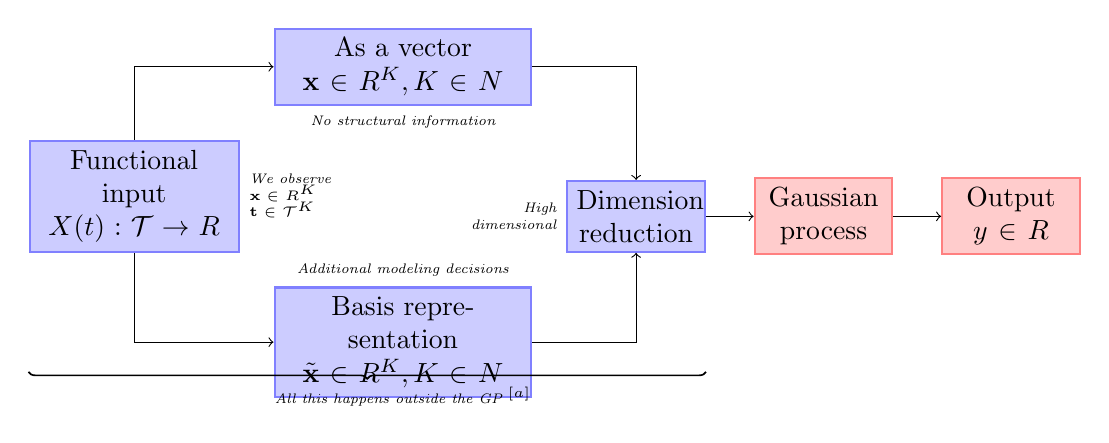
\begin{tikzpicture}
  [
  txtbox1/.style={rectangle,align=center,draw=blue!50,fill=blue!20,thick},
  txtbox2/.style={rectangle,align=center,draw=red!50,fill=red!20,thick},
  every label/.style={font=\itshape\tiny}
  ]

  \node (inp)  [txtbox1] at ( 0,  0) [text width=16ex]
  [label={[align=left]right:We observe \\ $\mathbf{x} \in \mathbb{R}^K$\\ $\mathbf{t}\in\mathcal{T}^K$}] {
    Functional input \\
    $X(t): \mathcal{T} \to \mathbb{R}$
  };
  \node (vec1) [txtbox1] [above right=4ex of inp]   [text width=20ex]
  [label=below:No structural information]{
    As a vector \\
    $\mathbf{x} \in \mathbb{R}^K, K \in \mathbb{N}$
  };
  \node (vec2) [txtbox1] [below right=4ex of inp]   [text width=20ex]
  [label=above:Additional modeling decisions]{
    Basis representation \\
    $\tilde{\mathbf{x}} \in \mathbb{R}^K, K \in \mathbb{N}$
  };

  \node (dred) [txtbox1] [above right=4ex of vec2] [text width=10ex]
  [label={[align=right]left:High\\dimensional}]
  {
    Dimension \\ reduction
  };

  \node (gp)   [txtbox2] [right=4ex of dred] [text width=10ex] {
    Gaussian \\ process
  };
  \node (out)  [txtbox2] [right=4ex of gp] [text width=10ex]  {
    Output \\ $y \in \mathbb{R}$
  };

  \node [below=6ex of vec2.north, label=below:All this happens outside the GP$~^{[a]}$] {
  };

  \draw [->] (inp.north) |- (vec1.west);
  \draw [->] (inp.south) |- (vec2.west);
  \draw [->] (vec1.east) -| (dred.north);
  \draw [->] (vec2.east) -| (dred.south);
  \draw [->] (dred.east) -- (gp.west);
  \draw [->] (gp.east)   -- (out.west);
  \path (inp.south west)
  edge[decorate,decoration={brace,mirror,raise=10ex},line width=.6pt]
  (inp.south west -| dred.south east);
\end{tikzpicture}

%%% Local Variables:
%%% mode: latex
%%% TeX-master: t
%%% End:


  \blankfootnote{
  % $~^{[1]}$\cite{muehlenstaedt2017,nanty2016,wang2017,tan2019,wang2019,betancourt2020,betancourt2020a,li2021} \,
  % $~^{[2]}$\cite{morris2012,kuttubekova2019}
%    $~^{[1]}$
  [a]
  Treat as vectors~\cite{iooss2009,nanty2016};
  reproject via splines~\cite{betancourt2020,betancourt2020a},
  functional principal component analysis~\cite{wang2017,wang2019},
  other basis representations~\cite{tan2019,li2021,striegel2022}\\
  \hspace{3.25ex}
  See also other attempts to incorporate the functional input structure into the
  GP~\cite{morris2012,muehlenstaedt2017,kuttubekova2019,Chen2021}
  \hyperlink{frm:litrev}{\resizebox{!}{1.5ex}{\beamergotobutton{appendix}}}
  }
\end{frame}

% Automatic Dynamic Relevance Determination ------------------------------------
\section{Automatic \textit{Dynamic} Relevance Determination \\
  {\tiny
    \href{https://doi.org/10.48550/arXiv.2209.00044}{arXiv:2209.00044}}
}

\begin{frame}
  \frametitle{Automatic Dynamic Relevance Determination}
  \framesubtitle{A framework for Gaussian Processes with functional inputs}

  \begin{align}
    y\in\mathcal{Y}
    &=\Reals \\
    X(t)\in\mathcal{X}
    &=\left\{X\colonfun\mathcal{T}\to\mathbb{R}, \int X(t)^2\mathrm{d}{t}<\infty\right\}
    \\
    t\in\mathcal{T}
    &=[0, 1]
      \only<2->{
      \\
    f
    &\hphantom{\colonfun\colonfun}
      \colonfun
      \hphantom{\colonfun\colonfun}\mathcal{X}\to\mathcal{Y} \\
    y_i
    &= f(X_i) \\
    f
    &\sim\mathcal{GP}(\cdot, \cdot)
      }
  \end{align}

  \blankfootnote{We assume that $t$ belongs in the unit interval w.l.o.g.}
\end{frame}

\begin{frame}
  \frametitle{Automatic Dynamic Relevance Determination}
  \framesubtitle{A framework for Gaussian Processes with functional inputs}

  \begin{align}
    \mathbf{y}
    &\sim \mathcal{N}\left(\mathbf{m}_f, \sigma_{f}^{2} \ \mathbf{R}_f
      + \sigma_{\varepsilon}^{2}\mathbf{I}\right) \\
    (\mathbf{m}_f)_i
    &= m_f(X_i) \\
    {\left(\mathbf{R}_f\right)}_{ij}
    &=
      \text{exp}\left\{
      -0.5 \phi^{-2} \ d_f(X_i, X_j)
      \right\}
      \only<2->{
    \\
    d_f(X_i, X_j)
    &= \int_{\mathcal{T}}
      \omega(t)
      {\left(X_i(t) - X_j(t) \right)}^2 dt
    \\
    \omega(t)
    &: \mathcal{T}\to\mathbb{R}^+
      }
  \end{align}

  \blankfootnote{
    $\sigma_{\varepsilon}^2 > 0$,
    $\sigma_{f}^2 > 0$,
    $\phi > 0$,
    $i, j = 1, \dots, N$,
    and $m_f(\cdot)$ is a mean function left unspecified for this presentation
  }
\end{frame}

\begin{frame}
  \frametitle{Automatic Dynamic Relevance Determination}
  \framesubtitle{From ARD to ADRD}

  %% tikz diagram
  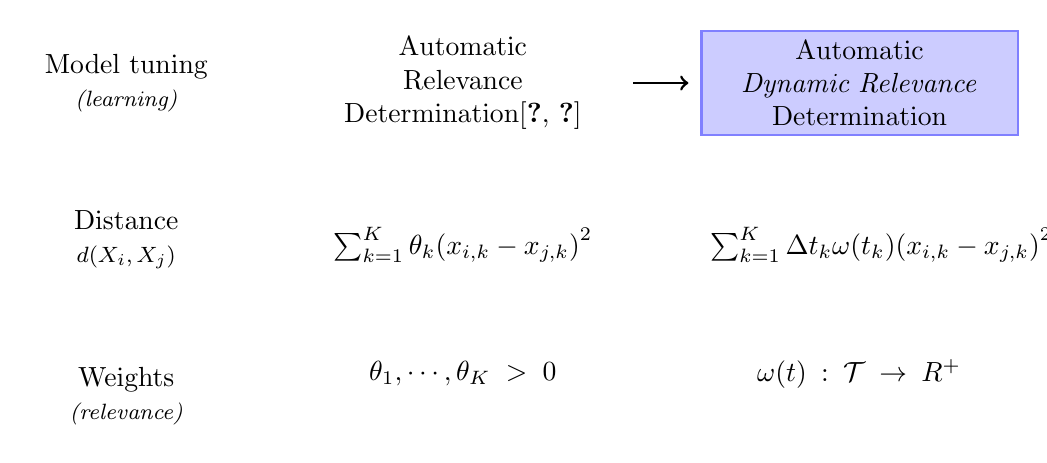
\begin{tikzpicture}
  [
  txtbox1/.style={rectangle,align=center,draw=blue!50,fill=blue!20,thick},
  every label/.style={font=\itshape\footnotesize}
  ]
  \tikzset{every node/.style={align=center}}
  \node (aspect1b)   at (0, 0)                        [text width=15ex] {
    Model tuning\\{\footnotesize \itshape (learning)}
  };
  \node (aspect2)    [below=of aspect1b]              [text width=15ex] {
    Distance\\{\footnotesize $d(X_i, X_j)$}
  };
  \node (aspect3)    [below=of aspect2]               [text width=15ex] {
    Weights\\{\footnotesize \itshape (relevance)}
  };
  %%%%%
  \node (solution1b) [right=of aspect1b]              [text width=25ex] {
    Automatic\\Relevance\\Determination\cite{neal1996,neal1998}
  };
  %%%%%
  \node (solution2b) [txtbox1] [right=of solution1b]  [text
  width=25ex]
  [visible on=<2->]{
    Automatic\\\textit{Dynamic Relevance}\\Determination
  };
  %%%%%
  \node (eq1b) [below=of solution1b] [text width=25ex] {
    % $\sum_{k=1}^K \frac{{(x_{i, k} - x_{j, k})}^2}{\ell_k^2}$
    $\sum_{k=1}^K \theta_k {(x_{i, k} - x_{j, k})}^2$
  };
  % \node (eq2b) [below=of solution2b] [text width=25ex]
  \node (eq2b) [right=of eq1b] [text width=25ex]
  [visible on=<2->]{
    % $\int_{\mathcal{T}}
    % \omega(t)
    % {\left(X_i(t) - X_j(t) \right)}^2 \mathrm{d}t$
    $\sum_{k=1}^K \Delta t_k \omega(t_k) {(x_{i, k} - x_{j, k})}^2$
  };
  %%%%%
  \node (par1b) [below=of eq1b] [text width=25ex]{
    % $\ell^{-2}_1, \cdots, \ell^{-2}_K > 0$
    $\theta_1, \cdots, \theta_K > 0$
  };
  % \node (par2b) [below=of eq2b] [text width=25ex]
  \node (par2b) [right=of par1b] [text width=25ex]
  [visible on=<2->]{
    $\omega(t): \mathcal{T} \to \mathbb{R}^+$
  };
  \draw[shorten >=1ex,shorten <=1ex,line width=1pt]
  [visible on=<2->] [->] (solution1b.east) -- (solution2b.west);
  % \draw[shorten >=1ex,shorten <=1ex,line width=1pt]
  % [visible on=<3->] [->] (eq1b.east) -- (eq2b.west);
  % \draw[shorten >=1ex,shorten <=1ex,line width=1pt]
  % [visible on=<4->] [->] (par1b.east) -- (par2b.west);
\end{tikzpicture}

%%% Local Variables:
%%% mode: latex
%%% TeX-master: t
%%% End:


  \only<2->{
    \blankfootnote{
      \hyperlink{frm:riemann}{\resizebox{!}{1.5ex}{\beamergotobutton{appendix}}}
      The Riemann approximation is used throughout this presentation
    }
  }
\end{frame}

\begin{frame}
  \frametitle{Automatic Dynamic Relevance Determination}
  \framesubtitle{A simple example}

  We want to predict $y_j | y_i, X_i(t), X_j(t)$ via a zero-mean Gaussian
  process for two observations $i, j$.

  \begin{align}
    \EV{y_j | y_i, X_i(t), X_j(t)}
    &=
    y_i e^{-\frac{1}{2}\phi^{-2} \int_\mathcal{T}
    {\omega(t) \left(X_i(t) - X_j(t)\right)}^2\,\mathrm{d}t} \\
    \VV{y_j | y_i, X_i(t), X_j(t)}
    &=
      \sigma_f^2
      (1 - e^{-\phi^{-2} \int_\mathcal{T}
    {\omega(t) \left(X_i(t) - X_j(t)\right)}^2\,\mathrm{d}t})
  \end{align}

  \begin{itemize}
  \item A prediction is generated by comparing the two inputs profiles
    everywhere, but \emph{especially} in higher weight index subspaces
  \item Input differences in index subspaces with little weight
    $\{t:\omega(t)\approx0\}$ will have limited to no impact on predictions
  \end{itemize}
\end{frame}

\begin{frame}
  \frametitle{Automatic Dynamic Relevance Determination}
  \framesubtitle{Framework goals}

  \begingroup
  \setbeamersize{description width=-\labelsep}
  \begin{description}
  \item[No dimension reduction] \mbox{}\\
    No need to lose information even for large $K$
  \item[Parsimony] \mbox{}\\
    $\omega(t)$ can be tuned with fewer parameters than \textsc{ARD}
  \item[Smoothness] \mbox{}\\
    Smooth relevance function to penalize erratic or noisy \textsc{ARD} patterns
    \\
    e.g., $X(t_{k_1})$, $X(t_{k_2})$ and
    $X(t_{k_3})$ having disparate weights despite $t_{k_1} < t_{k_2} <
    t_{k_3}$ being close on the index space for the scale of the physical
    problem
  \item[Interpretability] \mbox{}\\
    $\omega(t) | \mathbf{y}$ may provide information about the underlying
    physical process
  \end{description}
  \endgroup
\end{frame}

\begin{frame}
  \frametitle{Automatic Dynamic Relevance Determination}
  \framesubtitle{Other considerations}

  In principle, this framework is compatible with
  \begin{itemize}
  \item unregistered / unaligned observations
  \item correlation functions other than the squared exponential
  \item full and empirical Bayes, maximum likelihood, cross validation,
    other training paradigms
  \item big data approximations, e.g., local approximations
  \item distributed and GPU-accelerated computing
  \item smoothing models other than Gaussian Processes
  \end{itemize}
\end{frame}

% Microwave Limb Sounder -------------------------------------------------------
\section{NASA's Microwave Limb Sounder \\ {\small a case study} \\
  {\tiny
    \href{https://doi.org/10.48550/arXiv.2209.00044}{arXiv:2209.00044}}}

\begin{frame}[c]
  \frametitle{The science}
  \framesubtitle{Radiative transfer forward model}

  \begin{columns}[c]
    \begin{column}{0.2\textwidth}
      \begin{figure}
        \centering
        \includegraphics[height=8.5em]{inc/mls_aura}
        \caption*{
          \href{https://www.jpl.nasa.gov/missions/microwave-limb-sounder-mls}{\resizebox{!}{1.5ex}{\beamergotobutton{www}}}
          NASA JPL}
      \end{figure}
    \end{column}
    \begin{column}{0.7\textwidth}
      \begin{itemize}
      \item Computer model: forward
        model~\cite{read2006,schwartz2006,waters2006} estimates, or
        \emph{retrieves}, geophysical variables from electromagnetic radiation
      \item Planetwide, daily data products~\cite{liversey2020} and uncertainty
        experiments~\cite{turmon2019,braverman2021} rely on a myriad of runs
      \item Output: score for reflected sunlight around 190GHz~\cite{johnson2020}
      \item Functional input: atmospheric profiles over a vertical grid
      \item We consider some species in pressure regions expected to be
        well-informed by the measurements~\cite{liversey2020}
      \end{itemize}
    \end{column}
  \end{columns}
\end{frame}

\begin{frame}[c]
  \frametitle{Data}
  \framesubtitle{Atmospheric composition and radiance}

  \begin{figure}
    \centering
    \includegraphics[height=10em]{inc/mls_input_profiles}
  \end{figure}

  \begin{center}
    Radiance score variability seems associated with the tropopause Ozone
    concentration
  \end{center}

  \blankfootnote{
    $y\in\mathbb{R}$ scaled radiance score,
    $X(t)\in\mathbb{R}$ scaled concentration at $t$ \\
    \hspace{3.25ex}
    $t\in[0, 1]$ scaled reversed log pressure s.t.
    $t \to 0^{+}$ and $t \to 1^{-}$ as measurements near the tropopause and
    mesopause, respectively}
\end{frame}

\begin{frame}[c]
  \frametitle{Methods}
  \framesubtitle{Model}

  \begin{figure}
    \centering
    \includegraphics[height=10em]{inc/mls_weight_profiles}
  \end{figure}

  \begin{equation}
    \omega(t)
    =
    \text{exp}\left\{-(t - \tau)\lambda\kappa^s s\right\}
  \end{equation}

  % \begin{align}
  %   $\omega(t)
  %   &= \text{exp}\left\{-(t - \tau) \lambda\kappa^s s\right\}$ \\
  %   &=
  %   \begin{cases}
  %     \lambda_1 = \lambda\kappa^{-1}%
  %     & t < \tau \\
  %     \lambda_2 = \lambda\kappa%
  %     & t > \tau \\
  %   \end{cases}
  % \end{align}

  \blankfootnote{
    Space:
    $\omega(t): \mathcal{T} = [0, 1] \to (0, 1]$,
    $s = \text{sign}(t - \tau)$,
    $\tau\in[0,1]$,
    $\lambda > 0$,
    $\kappa > 0$ \\
    \hspace{3.25ex}
    Priors:
    $\indent\tau \sim \textsc{Beta}$,
    $\lambda \sim \textsc{N}^{+}$,
    $\log(\kappa) \sim \textsc{N}$
  }
\end{frame}

\begin{frame}
  \frametitle{Methods}
  \framesubtitle{Implementation}

  \begin{itemize}
  \item 8 training and 8 test complementary sets with 1,000 soundings each
  \item 7 plausible models
    \begin{itemize}
    \item viGP SE, ARD, FPCA, FFPCA
    \item fiGP Exponential ($\tau=0,\kappa=1$), SDE ($\kappa=1$), ADE (all free)
    \end{itemize}
  \item
    \hyperlink{frm:inference}{\resizebox{!}{1.5ex}{\beamergotobutton{appendix}}}
    Fully Bayesian inference
    \begin{itemize}
    \item Hamiltonian Monte Carlo~\cite[ch. 5]{brooks2011}
    \item NUTS algorithm~\cite{hoffman2014} via
      Stan~\cite{standevelopmentteam2021}
    \item 1 long chain~\cite{raftery1992}
    \item Extensive search for an initial value
    \item 500 post-warmup iterations
    \item 1,500 posterior samples
    \end{itemize}
  \item \hyperlink{frm:validation}{\resizebox{!}{1.5ex}{\beamergotobutton{appendix}}}
    Numerous out-of-sample validation statistics
  \end{itemize}
\end{frame}

\begin{frame}[c]
  \frametitle{Results}
  \framesubtitle{Posterior predictive validation}

  \begin{table}
    \adjustbox{width=.79\textwidth,center}{%
      \centering
      \begin{tabular}{lrrrrr|r}
        \toprule
        \input{inc/validation-statistics-RMSE}
      \end{tabular}
      \begin{tabular}{lrrrrr|r}
        \toprule
        \input{inc/validation-statistics-PPLD}
      \end{tabular}}
    \caption*{%
      Mean validation statistics:~RMSE (left) and negative PPLD (right).\\
      Smaller values are better. Bold is best in class. \\
      One model fit separately per input.
    }%
    \label{tab:validation-statistics-mini}
  \end{table}

  \blankfootnote{
    $
    \hat{v}_1
    = {\tilde{M}}^{-1} \sum_{{\tilde{m}}=1}^{{\tilde{M}}} N^{-\frac{1}{2}}
    \norm{%
      \EV{\bm{y}_{*} | \bm{X}, \bm{X}_{*}, \bm{y}, {\bm{\theta}}_{{\tilde{m}}}}
      - \bm{y}_{*}}
    $ \\
    \hspace{3.25ex}
    $
    \hat{v}_2 = {\tilde{M}}^{-1} \sum_{{\tilde{m}}=1}^{{\tilde{M}}}
    p(\bm{y}_{*} | \bm{X}, \bm{X}_{*}, \bm{y},
    {\bm{\theta}}_{{\tilde{m}}})
    $
 }
\end{frame}

\begin{frame}
  \frametitle{Results}
  \framesubtitle{Posterior for model interpretation}

  \begin{figure}
      \centering
    \includegraphics[height=18em]{inc/mls_weight_posterior_oaat.png}
  \end{figure}

  % Figure with posterior weights for fiGP

  % If you only did optimization, you'd only get the pluses. By running full
  % bayes, I get the uncertainty (interval)

  % Consider showing the as a continuous function

  % Consider one posterior sample
\end{frame}

\begin{frame}
  \frametitle{Results}
  \framesubtitle{Posterior for model comparison}

  \begin{figure}
    \centering
    \includegraphics[height=17em]{inc/mls_weight_posterior_vifi.pdf}
  \end{figure}

  \blankfootnote{In this slide only, we fix $\kappa = 1$ so that
    $\omega(t)$ is symmetrical}
\end{frame}

\begin{frame}
  \frametitle{Model}
  \framesubtitle{Multiple inputs}

  We want to model the radiance score as a function of multiple chemical
  species, namely H$_2$, O$_3$, N$_2$O, HNO$_3$, and temperature.
  \begin{equation}
    y = f(X^{(1)}, X^{(2)}, X^{(3)}, X^{(4)}, X^{(5)})
  \end{equation}

  Assume separability with one weight function per functional input
  \begin{equation}
    \mathrm{Cor}(y_i, y_j) = \prod_q^{Q = 5}
    \exp\left\{
      {\phi^{-2}}_{(q)}\int_\mathcal{T}
      \omega(t)^{(q)}{(X^{(q)}_{i}(t) - X^{(q)}_{j}(t))}^2\,\mathrm{d}t
    \right\}
  \end{equation}

  Use the integrated weight to gauge the contribution of each species
  \begin{equation}
    \Omega_q = \phi_{(q)}^{-2}\int_\mathcal{T}\omega^{(q)}(t)\,\mathrm{d}t
  \end{equation}
\end{frame}

\begin{frame}
  \frametitle{Results}
  \framesubtitle{Posterior for model interpretation}

  \begin{figure}
    \centering
    \includegraphics[height=11em]{inc/mls_weight_posterior.pdf}
  \end{figure}
  \vfill{}
  \begin{itemize}
  \item Validation: ADRD and ARD get $R^2 = .97$ out of sample
  \end{itemize}

  \blankfootnote{
    $
    p(\omega(t) | \bm{X}, \bm{y})
    \approx
    \{
    \omega_m(t) | \bm{X}, \bm{y}, \bm{\theta}_m
    : m = 1, \dots, M\}
    $
  }
\end{frame}

\begin{frame}
  \frametitle{Results}
  \framesubtitle{Which inputs are most relevant?}

  \begin{figure}
    \centering
    \includegraphics[height=15em]{inc/mls_weight_integral.pdf}
  \end{figure}

  \blankfootnote{
    Integrated weight:
    $
    \Omega = \phi^{-2}\int_\mathcal{T}\omega(t)\,\mathrm{d}t
    $,
    $
    p(\Omega | \bm{X}, \bm{y})
    \approx
    \{
    \Omega_m | \bm{X}, \bm{y}, \bm{\theta}_m
    : m = 1, \dots, M\}
    $
  }
\end{frame}

\begin{frame}
  \frametitle{Discussion}
  \framesubtitle{Short summary}

  \begin{itemize}
  \item ADRD and ARD perform similarly prediction-wise
  \item ADRD and ARD agree on the overall relevance patterns
  \item ADRD has $\sim15$ times fewer parameters to learn
  \item ADRD rules out erratic patterns in relevance
  \item ADRD posterior patterns are consistent with the underlying science
    \begin{itemize}
    \item Relevance within a chemical species over the vertical grid via the
      $\omega(t)$ function
    \item Relevance between chemical species via the integrated weight statistic
      $\Omega$
    \item \hyperlink{frm:pfdi}{\resizebox{!}{1.5ex}{\beamergotobutton{appendix}}} Patterns observed via relevance screening
    \end{itemize}
  \end{itemize}
\end{frame}

% Daily Erosion Project --------------------------------------------------------
\section{Daily Erosion Project \\ {\small a case study} \\
  {\tiny upcoming manuscript}}

\begin{frame}
  \frametitle{The science}
  \framesubtitle{Iowa losses the thickness of a dime in soil per year (1-billion
    dollar, .5\% GDP)}

  %% Detachment
  %% https://www.dailyerosion.org/map/#20211201/20221130/avg_loss/-93.10/42.09/7.766666666666668//0/
  %% Soil loss https://www.dailyerosion.org/map/#20211216/20221215/avg_delivery/-93.56/42.05/7.766666666666668//0/
  %% https://www.desmoinesregister.com/story/money/agriculture/2014/05/03/erosion-estimated-cost-iowa-billion-yield/8682651/
  %% July 4th
  \begin{figure}
    \centering
    \includegraphics[height=17em]{inc/dep_soilloss_map_20221215_168.png}
      \caption*{%
        \href{https://bit.ly/3HZyaRl}{\resizebox{!}{1.5ex}{\beamergotobutton{www}}}
        Interactive map from dailyerosion.org (change to hillslope soil loss)}
  \end{figure}
\end{frame}

\begin{frame}
  \frametitle{Data}
  \framesubtitle{How does landscape affect soil loss?}

  \begin{figure}
    \centering
    \includegraphics[height=17em]{inc/wepp_elevation_profiles}
    \caption*{
          \href{https://www.ars.usda.gov/midwest-area/west-lafayette-in/national-soil-erosion-research/docs/wepp/}{\resizebox{!}{1.5ex}{\beamergotobutton{www}}}
      Water Erosion Prediction Project version 2012.800
    }
  \end{figure}

  % {\tiny
  %   \href{https://www.ars.usda.gov/midwest-area/west-lafayette-in/national-soil-erosion-research/docs/wepp/}{\resizebox{!}{1.5ex}{\beamergotobutton{www}}}
  %     Water Erosion Prediction Project version 2012.800}
\end{frame}

\begin{frame}
  \frametitle{Data}
  \framesubtitle{Landscape characteristics and soil loss}

  \begin{itemize}
  \item Output: $y\in\mathbb{R}$ daily sediment delivery off-site (log kg/m)
  \item Inputs:
    \begin{itemize}
    \item Hillslope length: $x_1\in\mathbb{R}$ length (log m) of the overland flow
      element
    \item Mean slope: $x_2\in\mathbb{R}$ slope integral (log m/m) over the profile
    \item Slope profile: $X(t)\in\mathbb{R}$ slope steepness (log m/m) at $t$
    \item Normalized distance: $t\in[0, 1]$ from hilltop
    \item Discretization: $\{X(t_k) : t_k = k / 20, k = 1, \dots, 19\}$
    \item Climate, management, and soil parameters fixed constant
    \item Inputs are transformed to have approximately the same scale
    \end{itemize}
  \end{itemize}

  \vfill

  $\mathrm{Cor}(y_i, y_j) =
  \underbrace{\exp\{
    \int_\mathcal{T}
    \omega(t){(X_i(t) - X_j(t))}^2\,\mathrm{d}t\}
  }_{\mathrm{ADRD}}
  \times
  \underbrace{
    \vphantom{\int_\mathcal{T}}
      \exp\{\theta_1 {(x_{1i} - x_{1j})}^2\}
  \times
  \exp\{\theta_2 {(x_{2i} - x_{2j})}^2\}
  }_{\mathrm{ARD}}$
\end{frame}

\begin{frame}
  \frametitle{Methods}
  \framesubtitle{Model}

  % $d$ hillslope distance

  % $t = d / D$ distance normalized to 0, 1

  % $H(t)$ elevation at t

  % $X(t) = \partial{}H(t)\partial{}t$ Slope (m/m)

  % $x_1 = \log \int_{0}^d X(u)\mathrm{d}u$ Mean slope (m)

  % $x_2 = \log d$ Hillslope length (m)

  % $\log y$ Soil loss (mm)

  \begin{figure}
    \centering
    \includegraphics[height=10em]{inc/few_weight_profiles}
  \end{figure}

  \begin{equation}
    \log\omega(t)
    \label{eq:few-log}
    =\psi_{c,0} + \sum_{g = 1}^{G} \psi_{c,g}\cos\left(2\pi gt\right)
      + \sum_{g = 1}^{G} \psi_{s,g}\sin\left(2\pi gt\right)
  \end{equation}

  \blankfootnote{
    Space:
    $\psi_{c,g},\psi_{s,g}\in\Reals$, $G\in\mathbb{N}$ \\
    \hspace{3.25ex}
    Identifiability: (i) $\phi = 1$, (ii) $\psi_{c,0} = 0$,
    (iii) $\max_\mathcal{T}\omega(t) = 1$, or (iv)
    $\int_\mathcal{T}\omega(t)\dx{t} = 1$
  }
\end{frame}

\begin{frame}
  \frametitle{Methods}
  \framesubtitle{Implementation}

  \begin{itemize}
  \item 8 training and 8 test complementary sets with 300 landscapes each
  \item 4 plausible models
    \begin{itemize}
    \item Vector input with ARD
    \item Functional input with asymmetric double exponential, asymmetric
      squared exponential, and Fourier weights
    \end{itemize}
  \item
    \hyperlink{frm:inference}{\resizebox{!}{1.5ex}{\beamergotobutton{appendix}}}
    Fully Bayesian inference
    \begin{itemize}
    \item Hamiltonian Monte Carlo~\cite[ch. 5]{brooks2011}
    \item NUTS algorithm~\cite{hoffman2014} via
      Stan~\cite{standevelopmentteam2021}
    \item 1 long chain~\cite{raftery1992}
    \item Extensive search for an initial value
    \item 500 post-warmup iterations
    \item 1,500 posterior samples
    \end{itemize}
  \item \hyperlink{frm:validation}{\resizebox{!}{1.5ex}{\beamergotobutton{appendix}}}
    Numerous out-of-sample validation statistics
  \end{itemize}
\end{frame}

\begin{frame}
  \frametitle{Results}
  \framesubtitle{Posterior predictive validation}

  \begin{figure}
    \centering
    \includegraphics[height=16em]{inc/wepp_validation_summary_mini.pdf}
  \end{figure}

  \blankfootnote{
    $
    \hat{v}_1
    = {\tilde{M}}^{-1} \sum_{{\tilde{m}}=1}^{{\tilde{M}}} N^{-\frac{1}{2}}
    \norm{%
      \EV{\bm{y}_{*} | \bm{X}, \bm{X}_{*}, \bm{y}, {\bm{\theta}}_{{\tilde{m}}}}
      - \bm{y}_{*}}
    $ \\
    \hspace{3.25ex}
    $
    \hat{v}_2 = {\tilde{M}}^{-1} \sum_{{\tilde{m}}=1}^{{\tilde{M}}}
    p(\bm{y}_{*} | \bm{X}, \bm{X}_{*}, \bm{y},
    {\bm{\theta}}_{{\tilde{m}}})
    $
  }
\end{frame}

\begin{frame}
  \frametitle{Results}
  \framesubtitle{Posterior for model interpretation}

  \begin{figure}
    \centering
    \includegraphics[height=15em]{inc/wepp_weight_posterior_mini.pdf}
  \end{figure}

  \blankfootnote{
    $
    p(\omega(t) | \bm{X}, \bm{y})
    \approx
    \{
    \omega_m(t) | \bm{X}, \bm{y}, \bm{\theta}_m
    : m = 1, \dots, M\}
    $
  }
\end{frame}

\begin{frame}
  \frametitle{Results}
  \framesubtitle{Posterior for model interpretation}

  \begin{figure}
    \centering
    \includegraphics[height=15em]{inc/wepp_weight_integral_mini.pdf}
  \end{figure}

  \blankfootnote{
    Integrated weight:
    $
    \Omega = \int_\mathcal{T}\omega(t)\,\mathrm{d}t
    $,
    $
    p(\Omega | \bm{X}, \bm{y})
    \approx
    \{
    \Omega_m | \bm{X}, \bm{y}, \bm{\theta}_m
    : m = 1, \dots, M\}
    $
  }
\end{frame}

\begin{frame}
  \frametitle{Discussion}
  \framesubtitle{Short summary}

  \begin{itemize}
  \item ADRD and ARD perform similarly prediction-wise
  \item ADRD and ARD agree on the overall relevance patterns
  \item ADRD has better goodness of fit with fewer parameters
  \item ADRD seems to extract more information than ARD from the slope profile
  \item Relevance seems to be very smooth in this computer model, as expected
  \end{itemize}
\end{frame}

% Discussion -------------------------------------------------------------------
\begin{frame}
  \frametitle{Summary}
  \framesubtitle{My work}

  Toward a framework for Gaussian processes with functional inputs
  $Y = f(X_1(u), X_2(v), \dots, x_1, x_2, \dots)$
  \begin{itemize}
    \footnotesize
  \item Framework for Gaussian processes with functional inputs
  \item Multiple scalar, vector, and functional inputs
  \item Flexible functional weight forms: ALF, ASE, FEW
  \item \hyperlink{frm:validation}{\resizebox{!}{1.5ex}{\beamergotobutton{appendix}}}
    Analytical integral for piecewise linear inputs
  \item Case studies: Microwave Limb Sounder, Water Erosion Prediction Project
  \end{itemize}
  \vspace{3ex}

  Future work
  \begin{itemize}
    \footnotesize
  \item Functional of multiple indexes Y = f(X(u, v))
    (\href{https://psumodeling.github.io/Cycles/}{
      \resizebox{!}{1.5ex}{\beamergotobutton{www}}}
    Cycles model basin 4D geometry)
  \item Functional input with functional output $Y(u) = f(X(v))$
  \item Relevance profile $\omega(t)$ with multiple local maxima (MLS
    Temperature, mixture)
  \item DoE:~A design to learn $\omega(t)$? Use $\omega(t)$ to inform the
    design?
  \item Couple with local approximation (non-stationary, large matrices)
  \item How to bring ADRD to (D)NNs?
  \end{itemize}
\end{frame}

% Closing slides ---------------------------------------------------------------
\begin{frame}[c]
  \frametitle{Acknowledgments}
  \centering

  {\small
    Benjamin Neo, Jarad Niemi, Max D. Morris (ISU) \\
    Margaret Johnson, Joaquim Texeira, Microwave Limb Sounder team
    (JPL, Caltech) \\
    Rick Cruise, Brian Gelder, Daryl Hermann (ISU) \\
    C-CHANGE:~Science for a Changing Agriculture \\
    Foundation for Food and Agriculture Research
  }

  \vfill

  {\huge Thank you!}

  \vfill

  {\tiny References and extra slides on the back}

  \href{ldamiano@iastate.edu}{\beamergotobutton{mail}
    ldamiano@iastate.edu}

  \href{https://luisdamiano.github.io}{\beamergotobutton{www}
    https://luisdamiano.github.io}

  \href{https://github.com/luisdamiano/ANL22}{\beamergotobutton{repo}
    https://github.com/luisdamiano/ANL22}
\end{frame}

\appendix
\setbeamertemplate{bibliography item}{\insertbiblabel}
\begin{frame}[allowframebreaks]{References}
  \tiny
  \bibliographystyle{unsrt}
  \bibliography{references}
\end{frame}

% Appendix ---------------------------------------------------------------------
\section{Appendix}

\begin{frame}%
  \label{frm:litrev}
  \frametitle{Literature review}

  Computer experiment with functional inputs $X(t):
  \mathcal{T}\to\mathbb{R}$ \\
  input quantities varying over a continuum typically modeled as function of
  some index

  \begin{itemize}
  \item Treat input as vectors~\cite{iooss2009}
  \item Transform input to vectors, e.g.,
    splines~\cite{betancourt2020,betancourt2020a}, principal component
    analysis~\cite{nanty2016}, functional principal component
    analysis~\cite{wang2017,wang2019}, among other basis
    functions~\cite{tan2019,li2021,striegel2022}
  \item A weight function for time-varying inputs and outputs~\cite{morris2012}
  \item A weight function for functional inputs with an $L^2$ norm approximated
    via splines~\cite{muehlenstaedt2017}
  \item A lengthscale function modeled via trigonometric basis
    functions~\cite{kuttubekova2019}
  \item A lengthscale for the functional input frequency~\cite{Chen2021}
  \end{itemize}

  \vfill{}
  Although functional input computer experiments are not uncommon,
  general methodology for functional input Gaussian processes is limited
\end{frame}

\begin{frame}%
  \label{frm:riemann}
  \frametitle{Integral approximation}

  We want to compute
  \begin{equation}
    I = \int_\mathcal{T}\omega(t){(X_i(t) - X_j(t))}^2\,\mathrm{d}t
  \end{equation}

  Define
  \begin{align}
    \Delta t_k
    &= t_{k} - t_{k - 1} \\
    D_{i,j,k}
    &= \omega(t_{k}) {\left(x_{i, k} - x_{j, k}\right)}^2
  \end{align}

  Trapezoidal approximation
  \begin{equation}
    I\approx
    \sum_{k = 2}^{K}
    \Delta t_k
    \frac{D_{i, j, k} + D_{i, j, k - 1}}{2}
  \end{equation}

  Since
  $S_k = e^{-\Delta t_k D_{i, j, k}}$ is positive semidefinite for fixed $k$, so
  is the product $S = \prod_{k} S_k$.

  \blankfootnote{See~\cite{muehlenstaedt2017} for a B-spline
    approach}
\end{frame}

\begin{frame}%
  \label{frm:piecewise}
  \frametitle{Analytical solution to piecewise linear inputs}

  \newcommand{\calT}{\mathcal{T}}
  \newcommand{\dt}{\, \mathrm{d}t}
  \newcommand{\du}{\, \mathrm{d}u}
  \newcommand{\dv}{\, \mathrm{d}v}
  \newcommand{\w}{\omega}
  \newcommand{\dotsq}{{\left[d(t)\right]}^2}
  \newcommand{\fall}{\,~\forall~\,}

  Let $\w(t): \calT \to \mathbb{R}_0^+$ be a weight function and $X_i(t),
  X_j(t): \calT \to \mathbb{R}$ be two functional input profiles over an index
  space $\calT$. Define $d_{ij}(t) = X_i(t) - X_j(t)$. We want to find $ I_{ij}
  \coloneqq \int_{\calT} \w(t) \, {\left[d_{ij}(t)\right]}^2 \dt$. We set
  $\calT = [0, 1]$ and consider the integral over the index space for any
  partition $T = \left\{ t_k: t_0 = 0 \le t_1 < \cdots < t_K \le t_{K+1} = 1
  \right\}$. We drop the subindexes $i$, $j$ for readability.
  \begin{align}
  I
  &=\int_0^1 \w(t) \, \dotsq \dt \label{eq:fnorm-direct} \\
  &=\sum_{k = 1}^{K + 1}
    \underbrace{
    \int_{t_{k-1}}^{t_k} \w(t) \, \dotsq
    \dt}_{C_k} \label{eq:fnorm-direct-pw}
  \end{align}
  % https://www.wolframalpha.com/input?i=Integrate%5Bw+*+%28a+%2B+b+*+t%29%5E2%2C+t%5D
  If $X(t)$ and $\omega(t)$ are piecewise linear and constant over $[t_{k-1},
  t_{k}]$, respectively, the integrand in $\cref{eq:fnorm-direct-pw}$ becomes
  $\omega(t) {(a + bt)}^2$ for $a,b\in\mathbb{R}$ and $C_k =
  {(3b)}^{-1}\omega(t_k)
  \left[
    {(a + b t_k)}^3 -
    {(a + b t_{k-1})}^3
  \right]
  $.
\end{frame}

\begin{frame}%
  \label{frm:inference}
  \frametitle{Fully Bayesian inference}

  \begin{itemize}
  \item We denote the parameter vector by $\bm{\theta} =
    (\bm{\theta}_{d}, \sigma_f^2, \sigma_{\varepsilon}^2)$, where
    $\bm{\theta}_{d}$ encompasses the unknowns for a specific choice of
    $d(X_i, X_j)$, e.g., $\bm{\theta}_{d} = (\phi, \lambda, \kappa, \tau)$.
  \item We generally recommend the following independent weakly informative
    priors for cases where there is no domain-specific information about
    the relevance profile:
    %
    $\phi \sim \textsc{InvGamma}(\cdot, \cdot)$,
    $\tau \sim \textsc{Beta}(\cdot, \cdot)$,
    $\lambda \sim \textsc{N}^{+}(\cdot, \cdot)$,
    $\log(\kappa) \sim \textsc{N}(\cdot, \cdot)$,
    $\phi\sim\textsc{N}(\cdot, \cdot)$
    for the fiGP parameters, and
    $\sigma_f, \sigma_{\varepsilon} \iid \textsc{N}^{+}(\cdot, \cdot)$
    for the standard deviation parameters.
  \item The choice
    of prior for $\phi$ is motivated by the fact that values extremely
    close to zero or large may lead to numerical issues due to posterior
    density flattening.
  \item Let $\mathbf{X}$ be training input matrix, $\mathbf{m}_y =
    m_y(\mathbf{X})$ the mean vector with %elements
    ${(\mathbf{m}_y)}_{i} = m_y(\mathbf{x}_i)$, and $\mathbf{S}_y =
    s_y(\mathbf{X})$ the covariance matrix with %elements
    ${(\mathbf{S}_y)}_{i, j} = s_y(X_i, X_j | {\bm{\theta}})$.
  \item Draw samples from the posterior $\bm{\theta}_m\sim\log p(\bm{\theta} |
    \mathbf{y}, \mathbf{X})$, $m = 1, \dots, M\in\mathbb{N}$
  \end{itemize}
  \begin{align}
    \label{eq:margina-likelihood}
    \log p(\mathbf{y} | \mathbf{X}, \bm{\theta})
    =& -\frac{1}{2}
       {(\mathbf{y} - \mathbf{m}_y)}^\top
       {\mathbf{S}_y}^{-1}
       {(\mathbf{y} - \mathbf{m}_y)}
       -\frac{1}{2}
       \log | \mathbf{S}_y |
       - \frac{n}{2} \log 2\pi \\
    \label{eq:parameter-posterior}
    \log p(\bm{\theta} | \mathbf{y}, \mathbf{X})
    \propto&
             \log p(\mathbf{y} | \mathbf{X}, \bm{\theta}) +
             \log p(\bm{\theta}).
  \end{align}
\end{frame}

\begin{frame}%
  \label{frm:validation}
  \frametitle{Validation statistics}

  \newcommand{\predmean}{\hat{\mathbf{m}}^{y}_*}
  \newcommand{\predvar}{\hat{\mathbf{S}}^{y}_*}
  \newcommand{\postpred}{\hat{p}^{y}_*}

  \begin{itemize}
  \item   Let
    $\hat{\mathbf{m}} = \predmean = \{\hat{m}_{*n}: n = 1, \dots, N\} =
    \EV{\mathbf{y}_* | \mathbf{y}, \mathbf{X}, \mathbf{X}_*}$
    and
    $\hat{\mathbf{S}} = \predvar = \VV{\mathbf{y}_* |
      \mathbf{y}, \mathbf{X}, \mathbf{X}_*}$
    be the predictive mean vector and covariance matrix.
  \item  Define the
    prediction error vector $\mathbf{e} = \mathbf{e}_{*}^{y} =
    \mathbf{y}_{*} - \hat{\mathbf{m}}$.
  \item Define the square Mahalanobis distance $D^2
    = \mathbf{e}^{\transp} \hat{\mathbf{S}}^{-1} \mathbf{e}$.
  \item Define the point-wise 95\% coverage indicator variable
    $I_{n} = 1$ if $y_{*n} \in \hat{m}_{*n} \pm 1.96
    {\hat{S}_{nn}}^{-\frac{1}{2}}$.
  \item   Let $\bar{y}_* = N^{-1} \sum_{n=1}^{N} y_{*n}$ be the test output
    mean.
  \end{itemize}

  \begin{center}
    \begin{tabular}{lrl}
      RMSE
      & $v_{\textsc{RMSE}}$ =
      & $N^{-\frac{1}{2}} \norm{\mathbf{e}}$ \\
      $R^2$
      & $v_{\textsc{R2}} $ =
      & $1 -%
        \norm{\mathbf{e}}^{2}
        \norm{\mathbf{y}_* - \bar{y}_*}^{-2}$ \\
      PPLD
      & $v_{\textsc{PPLD}}$ =
      & $
        -\frac{1}{2} \log \lvert \hat{\mathbf{S}} \rvert
        -D^2
        -\frac{n}{2} \log 2 \pi
        $
      \\
      CRPS
      & $v_{\textsc{CRPS}}$ =
      & $
        -\log \lvert \hat{\mathbf{S}} \rvert%
        -D^2
        $
      \\
      Nominal coverage
      & $v_{\textsc{COV95}}$ =
      & $N^{-1} \sum_{n = 1}^{N} I_{n}$
    \end{tabular}
  \end{center}
\end{frame}

\begin{frame}%
  \label{frm:pdfi}
  \frametitle{Dynamic relevance screening}

  \begin{itemize}
  \item We want to study the sensitivity of predictive accuracy to the
    information contained in different index subspaces
  \item We quantify the change in the validation statistics as we permute pieces
    of the input profile
  \item Let
    $\left\{\mathrm{T}_u\right\}_{u=1}^{U}, U \in \mathbb{N}$ form a
    partition of the index space $\mathcal{T}$.
  \item Let $\underline{\mathbf{x}}_{i,u} = [\mathbf{x}_{i,1}\cdots
    \mathbf{x}_{i',u}\cdots\mathbf{x}_{i,U}]$ be the corrupted input vector
    where $i' \ne i$ is chosen by random permutation, and
    $\underline{\mathbf{X}}_u$ the corrupted input matrix
  \item Train an $d_{\textsc{ARD}}(\cdot)$ model with $\theta_k > 0 \
    \forall \ k = 1, \dots K$ on $\mathbf{X}$
  \item Validated on
    $\underline{\mathbf{X}}_{*u}$ instead of $\mathbf{X}_{*}$
  \item Compare the validation statistic
    produced with the corrupted test input matrix to the
    reference point via the deterioration statistic $\Delta_{u} =
    \underline{v}_{u} - v$.
  \item The higher the increase in the loss statistic due to the permutation
    in the input block associated with the $u$-th index interval, the more
    reliant prediction accuracy is on the corresponding index
    subspace.
  \end{itemize}
\end{frame}

\end{document}
